\section{Sampling}

\textbf{Sampling} is the process of converting a continuous-time signal into a discrete-time signal by measuring the signal's value at specific, uniformly spaced time instants. In the context of digital signal processing and computer vision, sampling is fundamental because real-world signals (such as images, sounds, or sensor measurements) are continuous in nature, but computers can only process discrete, finite sets of values.

The sampling process involves taking "snapshots" of a continuous signal at regular intervals, creating a sequence of discrete values that represent the original signal at those specific moments in time. The rate at which these samples are taken is called the \textbf{sampling frequency} or \textbf{sampling rate}, typically denoted as $f_s$ and measured in samples per second (Hz). The time interval between consecutive samples is called the \textbf{sampling period} $T_s = 1/f_s$.

A critical question in sampling theory is: \textit{How fast must we sample a signal to ensure that we can perfectly reconstruct the original continuous signal from its discrete samples?} This question is answered by the Nyquist-Shannon sampling theorem, which establishes the minimum sampling rate required for perfect reconstruction.

\subsection{The Nyquist-Shannon Sampling Theorem}

The Nyquist-Shannon sampling theorem, also known as the sampling theorem, is a fundamental principle in signal processing and digital image processing. It establishes the conditions under which a continuous signal can be perfectly reconstructed from its discrete samples.

\subsubsection{Statement of the Theorem}

\begin{theorem}[Nyquist-Shannon Sampling Theorem]
If a function $x(t)$ contains no frequencies higher than $B$ hertz, it is completely determined by giving its ordinates at a series of points spaced $\frac{1}{2B}$ seconds apart. In other words, a band-limited signal can be perfectly reconstructed from its samples if the sampling frequency $f_s$ satisfies:
\begin{equation}
f_s \geq 2f_{\text{max}}
\label{eq:nyquist}
\end{equation}
where $f_{\text{max}}$ is the highest frequency component in the signal. The frequency $f_N = \frac{f_s}{2}$ is called the \textbf{Nyquist frequency}, and $2f_{\text{max}}$ is called the \textbf{Nyquist rate}.
\end{theorem}

\begin{tcolorbox}[colback=blue!5!white, colframe=blue!75!black, title=\textbf{Curious Fact: Frequency and Period Relationship}]
The relationship between frequency $f$ and period $T$ is fundamental in signal processing:
\begin{align}
f &= \frac{1}{T} \label{eq:freq_period} \\
T &= \frac{1}{f} \label{eq:period_freq}
\end{align}
where:
\begin{itemize}
    \item $f$ is the frequency (measured in hertz, Hz, or cycles per second)
    \item $T$ is the period (measured in seconds, s, or time per cycle)
\end{itemize}
This means that frequency and period are inversely related: higher frequency corresponds to shorter period, and vice versa. For example, if a signal has a frequency of $f = 10$ Hz, its period is $T = \frac{1}{10} = 0.1$ seconds. In the context of sampling, the sampling period $T_s$ and sampling frequency $f_s$ are related by $T_s = \frac{1}{f_s}$.
\end{tcolorbox}

\subsection{Understanding Sampling in the Time Domain}

To understand the theorem, consider a continuous signal $x(t)$ that we wish to sample at regular intervals. The sampling process converts the continuous-time signal into a discrete-time signal by taking samples at uniformly spaced time instants. This relationship is mathematically expressed as:

\begin{equation}
x[n] = x(t_n), \quad t_n = nT_s, \quad n \in \mathbb{Z}, \quad T_s \in \mathbb{R}
\label{eq:sampling}
\end{equation}

where:
\begin{itemize}
    \item $x[n]$ is the discrete-time signal (sequence of samples)
    \item $x(t_n)$ is the value of the continuous signal at time instant $t_n$
    \item $n$ is an integer index representing the sample number
    \item $T_s$ is the sampling period (time interval between consecutive samples)
    \item $f_s = \frac{1}{T_s}$ is the sampling frequency
\end{itemize}

Figure~\ref{fig:sampling_process} illustrates this sampling process, showing how a continuous signal is converted into a discrete sequence of samples.

\begin{figure}[H]
    \centering
    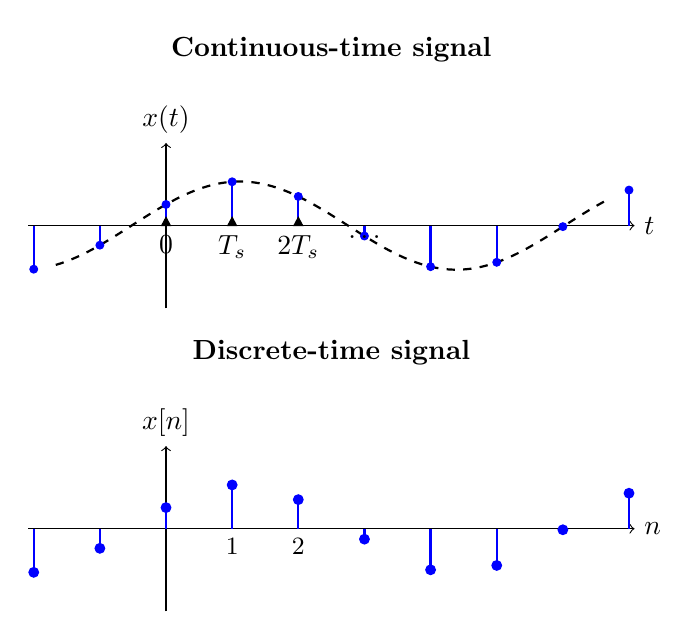
\begin{tikzpicture}[scale=0.7]
        % Define sampling period
        \def\Ts{1.2}
        \def\amplitude{0.8}
        
        % Continuous signal plot
        \begin{scope}[yshift=5.5cm]
            \draw[->] (-2.5,0) -- (8.5,0) node[right] {$t$};
            \draw[->] (0,-1.5) -- (0,1.5) node[above] {$x(t)$};
            \node[above] at (3,2.8) {\textbf{Continuous-time signal}};
            
            % Draw continuous signal (sine wave)
            \draw[thick, dashed, black] plot[smooth, domain=-2:8, samples=200] (\x, {\amplitude*sin(deg(\x*0.8 + 0.5))});
            
            % Sampling points
            \foreach \n in {-2,-1,0,1,2,3,4,5,6,7} {
                \pgfmathsetmacro{\t}{\n * \Ts}
                \pgfmathsetmacro{\y}{\amplitude*sin(deg(\t*0.8 + 0.5))}
                \draw[blue, thick] (\t,0) -- (\t,\y);
                \filldraw[blue] (\t,\y) circle (2pt);
            }
            
            % Sampling period markers on x-axis
            \node[below] at (0,0) {$0$};
            \node[below] at (\Ts,0) {$T_s$};
            \node[below] at (2*\Ts,0) {$2T_s$};
            \node[below] at (3*\Ts,0) {$\ldots$};
            
            % Diamond markers (manually drawn)
            \filldraw[black] (0,0.15) -- (0.08,0) -- (0,0) -- (-0.08,0) -- cycle;
            \filldraw[black] (\Ts,0.15) -- (\Ts+0.08,0) -- (\Ts,0) -- (\Ts-0.08,0) -- cycle;
            \filldraw[black] (2*\Ts,0.15) -- (2*\Ts+0.08,0) -- (2*\Ts,0) -- (2*\Ts-0.08,0) -- cycle;
        \end{scope}
        
        % Discrete signal plot
        \begin{scope}
            \draw[->] (-2.5,0) -- (8.5,0) node[right] {$n$};
            \draw[->] (0,-1.5) -- (0,1.5) node[above] {$x[n]$};
            \node[above] at (3,2.8) {\textbf{Discrete-time signal}};
            
            % Draw discrete samples (at same x-positions as continuous graph)
            \foreach \n in {-2,-1,0,1,2,3,4,5,6,7} {
                \pgfmathsetmacro{\t}{\n * \Ts}
                \pgfmathsetmacro{\y}{\amplitude*sin(deg(\t*0.8 + 0.5))}
                \draw[blue, thick] (\t,0) -- (\t,\y);
                \filldraw[blue] (\t,\y) circle (2.5pt);
            }
            
            % Label x-axis with integer indices (only 1 and 2, at same positions as continuous)
            \node[below] at (\Ts,0) {\small $1$};
            \node[below] at (2*\Ts,0) {\small $2$};
        \end{scope}
    \end{tikzpicture}
    \caption{Sampling process: conversion from continuous-time signal $x(t)$ to discrete-time signal $x[n]$. The top plot shows the continuous signal with sampling instants marked, and the bottom plot shows the resulting discrete sequence.}
    \label{fig:sampling_process}
\end{figure}

\subsection{Signal Reconstruction with Sinc Interpolation}

Once a signal has been sampled according to the Nyquist-Shannon theorem, the original continuous signal can be perfectly reconstructed from its discrete samples. This reconstruction is achieved through \textbf{sinc interpolation}, which uses the sinc function to interpolate between sample points.

The sinc function is defined as:
\begin{equation}
\text{sinc}(t) = \frac{\sin(\pi t)}{\pi t}
\label{eq:sinc}
\end{equation}
with the special case $\text{sinc}(0) = 1$ (by L'Hôpital's rule).

The reconstruction formula, also known as the \textbf{Whittaker-Shannon interpolation formula}, expresses the continuous signal $x(t)$ as a weighted sum of sinc functions centered at each sample point:
\begin{equation}
x(t) = \sum_{n=-\infty}^{\infty} x[n] \cdot \text{sinc}\left(\frac{t - nT_s}{T_s}\right)
\label{eq:reconstruction}
\end{equation}

where:
\begin{itemize}
    \item $x[n]$ are the discrete samples
    \item $T_s$ is the sampling period
    \item Each sinc function is centered at a sampling instant $nT_s$
    \item The sinc function has zeros at all other sampling instants, ensuring that $x(t)$ equals $x[n]$ at $t = nT_s$
\end{itemize}

This reconstruction works because:
\begin{enumerate}
    \item At each sampling instant $t = nT_s$, only the sinc function centered at that point contributes (all others are zero), so $x(nT_s) = x[n]$.
    \item Between sampling points, the sinc functions smoothly interpolate the signal values.
    \item In the frequency domain, the sinc function acts as an ideal low-pass filter, removing all frequency components above the Nyquist frequency while preserving those below it.
\end{enumerate}

\begin{tcolorbox}[colback=blue!5!white, colframe=blue!75!black, title=\textbf{Curious Fact: Band-Limited Signals and Perfect Reconstruction}]
Since sinc interpolation acts as a low-pass filter (removing all frequencies above the Nyquist frequency $f_N = f_s/2$), if we have a band-limited signal with maximum frequency $f_{\text{max}}$ lower than the Nyquist frequency, then no frequencies are going to be removed and therefore, the result is a theoretically perfect reconstruction.
\end{tcolorbox}

\subsection{Aliasing}

\textbf{Aliasing} is a distortion phenomenon that occurs when a signal is sampled at a rate that is too low (below the Nyquist rate). When aliasing occurs, high-frequency components of the signal are "folded back" or "aliased" into lower frequencies, making them indistinguishable from actual low-frequency components in the sampled signal.

\subsubsection{Why Aliasing Occurs}

In the frequency domain, sampling creates periodic replicas of the signal's spectrum at integer multiples of the sampling frequency. When the sampling frequency $f_s$ is less than $2f_{\text{max}}$, these replicas overlap. The overlapping high-frequency components appear as lower frequencies in the sampled signal, causing aliasing.

For example, consider a signal with frequency $f = 8$ Hz sampled at $f_s = 10$ Hz:
\begin{itemize}
    \item The Nyquist frequency is $f_N = f_s/2 = 5$ Hz
    \item The signal frequency (8 Hz) is above the Nyquist frequency
    \item The aliased frequency is $f_{\text{alias}} = f_s - f = 10 - 8 = 2$ Hz
    \item The sampled signal incorrectly appears to have a 2 Hz component instead of the original 8 Hz
\end{itemize}

\subsubsection{Consequences of Aliasing}

Once aliasing occurs, the original signal cannot be perfectly reconstructed because the high-frequency information has been irretrievably mixed with lower frequencies. This is why the Nyquist-Shannon theorem requires sampling at or above the Nyquist rate to ensure perfect reconstruction.

\begin{tcolorbox}[colback=blue!5!white, colframe=blue!75!black, title=\textbf{Curious Fact: The Wagon Wheel Effect}]
A classic example of aliasing in everyday life is the \textbf{wagon wheel effect} (also known as the stroboscopic effect) seen in videos. When a wheel with spokes rotates at a certain speed and is filmed at a fixed frame rate, the wheel can appear to rotate backward, slowly, or even stand still. This occurs because the wheel's rotation frequency is being undersampled by the camera's frame rate. The high-frequency rotation is aliased into a lower apparent frequency, creating the illusion of reverse or slow motion. This is a temporal aliasing effect, where time (rather than space) is being sampled.
\end{tcolorbox}

These are the three different sampling scenarios:

\begin{itemize}
    \item \textbf{Adequate sampling} ($f_s > 2f_{\text{max}}$): The signal can be perfectly reconstructed.
    \item \textbf{Nyquist rate sampling} ($f_s = 2f_{\text{max}}$): The minimum sampling rate that theoretically allows perfect reconstruction.
    \item \textbf{Insufficient sampling} ($f_s < 2f_{\text{max}}$): Aliasing occurs, and the original signal cannot be recovered.
\end{itemize}


\subsection{Exercise: Determining Minimum Sampling Rate}

Consider the following signal:
\begin{equation}
x(t) = \cos(100\pi t) + \sin(200\pi t) + \cos(500\pi t + \pi/4) + 7
\label{eq:exercise_signal}
\end{equation}

\textbf{Problem:} Determine the minimum sampling rate required to perfectly reconstruct this signal.

\textbf{Solution:}

To find the minimum sampling rate, we need to identify the maximum frequency component in the signal. Let's analyze each term:

\begin{itemize}
    \item $\cos(100\pi t)$: 
    \begin{align*}
    \text{Angular frequency: } \omega_1 &= 100\pi \text{ rad/s} \\
    \text{To convert to frequency: } f_1 &= \omega_1 \times \frac{1 \text{ cycle}}{2\pi \text{ rad}} \\
    &= 100\pi \text{ rad/s} \times \frac{1 \text{ cycle}}{2\pi \text{ rad}} \\
    &= \frac{100\cancel{\pi \text{ rad}}/\text{s} \times 1 \text{ cycle}}{2\cancel{\pi \text{ rad}}} \\
    &= \frac{100}{2} \frac{\text{cycle}}{\text{s}} = 50 \text{ cycles/s} = 50 \text{ Hz}
    \end{align*}
    
    \item $\sin(200\pi t)$: $f_2 = \frac{200\pi}{2\pi} = 100$ Hz
    
    \item $\cos(500\pi t + \pi/4)$: $f_3 = \frac{500\pi}{2\pi} = 250$ Hz
    
    \item $7$: This is a constant (DC component) with frequency $f_0 = 0$ Hz
\end{itemize}

The maximum frequency in the signal is $f_{\text{max}} = 250$ Hz (from the $\cos(500\pi t + \pi/4)$ term).

According to the Nyquist-Shannon theorem, the minimum sampling rate (Nyquist rate) is:
\begin{equation}
f_s \geq 2f_{\text{max}} = 2 \times 250 = 500 \text{ Hz}
\end{equation}

Therefore, the minimum sampling rate required is \textbf{500 Hz}.

Figure~\ref{fig:aliasing_exercise} demonstrates the signal reconstruction process using \textbf{sinc interpolation} (Whittaker-Shannon interpolation formula) for three different sampling scenarios. The reconstruction is performed using the formula:
\begin{equation}
x(t) = \sum_{n=-\infty}^{\infty} x[n] \cdot \text{sinc}\left(\frac{t - nT_s}{T_s}\right)
\end{equation}
where $\text{sinc}(t) = \frac{\sin(\pi t)}{\pi t}$ and $T_s = 1/f_s$ is the sampling period.

Each row of the figure shows three plots: (1) the original continuous signal, (2) the sampled signal with sample points marked, and (3) the reconstructed signal using sinc interpolation overlaid with the original for comparison. The three rows correspond to:
\begin{itemize}
    \item \textbf{Adequate sampling} ($f_s = 600$ Hz $> 2f_{\text{max}}$): The reconstructed signal perfectly matches the original, demonstrating perfect reconstruction when sampling above the Nyquist rate.
    \item \textbf{Nyquist rate sampling} ($f_s = 500$ Hz $= 2f_{\text{max}}$): The reconstructed signal matches the original, showing that the Nyquist rate is the theoretical minimum for perfect reconstruction.
    \item \textbf{Insufficient sampling} ($f_s = 300$ Hz $< 2f_{\text{max}}$): The reconstructed signal does not match the original due to aliasing, demonstrating that perfect reconstruction is impossible when sampling below the Nyquist rate.
\end{itemize}

\begin{figure}[H]
    \centering
    \includegraphics[width=0.95\textwidth]{img/aliasing_exercise.png}
    \caption{Signal reconstruction using sinc interpolation for $x(t) = \cos(100\pi t) + \sin(200\pi t) + \cos(500\pi t + \pi/4) + 7$ with $f_{\text{max}} = 250$ Hz. Each row shows: original signal (left), sampled signal (center), and reconstructed signal using sinc interpolation (right). The three rows demonstrate adequate sampling (600 Hz), Nyquist rate (500 Hz), and insufficient sampling (300 Hz) where aliasing prevents perfect reconstruction.}
    \label{fig:aliasing_exercise}
\end{figure}
